\documentclass[prb,9pt,notitlepage]{revtex4-1}
%\documentclass[a4paper,twocolumn,9pt]{article}

%\usepackage{geometry}
%\geometry{a4paper,top=2.5cm,bottom=2cm,inner=1.5cm,outer=1.5cm}

\usepackage{mwe}% just for the example content
\usepackage{color}
\usepackage{latexsym,amsmath}
\usepackage{physics}
\usepackage{listings}
\usepackage[dvipsnames]{xcolor}
\usepackage{parskip}
\usepackage{hyperref}
\usepackage{amsmath}
\usepackage{bbm}
%\usepackage{dblfloatfix}
%\usepackage{subfig}
\definecolor{linkcolor}{rgb}{0,0,0.65}%hyperlink
\definecolor{shadecolor}{rgb}{0.93, 0.93, 0.93}
%\usepackage[pdftex,colorlinks=true, pdfstartview=FitV, linkcolor= linkcolor, citecolor= linkcolor, urlcolor= linkcolor, hyperindex=true,hyperfigures=true]{hyperref} %hyperlink%
%\usepackage[backend=biber, sorting=ynt]{biblatex}
%\usepackage{ragged2e} % to justify caption
%\addbibresource{bibliography.bib}
 \usepackage{booktabs}

\usepackage[T1]{fontenc}
\usepackage{xcolor}
\usepackage{lmodern}
\usepackage{listings}
\lstset{language=[95]Fortran,
  backgroundcolor=\color{shadecolor},
  basicstyle=\ttfamily,
  keywordstyle=\color{blue},
  commentstyle=\color{gray},
  stringstyle=\color{red},
  showstringspaces=false
  %morecomment=[l]{!\ }% Comment only with space after !
}

\usepackage{tabularx}

\usepackage{fancyhdr}
\pagestyle{fancyplain}% <- use fancyplain instead fancy
\fancyhf{}
\fancyhead[R]{\today}
\fancyhead[L]{Alessandro Lambertini}
\fancyfoot[L]{Quantum information and computing}
\fancyfoot[C]{Report 2}
\fancyfoot[R]{\thepage}

\renewcommand{\headrulewidth}{0pt}

\usepackage{float}
\usepackage{siunitx}




\begin{document}
\title{Quantum information and computing: Exercises report, week 10. Quantum Ising Model and Real Space Renormalization Group }

\author{Alessandro Lambertini}


\date{\today}

\begin{abstract}
Through the exercise of this week,  we study from a numerical perspective the 1-D quantum Ising model in a transverse field, but this time by means of the RSRG algorithm. We implement the algorithm and we study the ground state of the system for different values of the interaction strenght $\lambda$.
\end{abstract}

\maketitle

\section{Theory}
The Hamiltonian that describes properly our system is the same of last week assignment:
\begin{equation}
  H = \lambda\sum_{i=1}^N \sigma_z^{(i)} + \sum_{i=1}^{N-1}\sigma_x^{i+1}\sigma_x^{i}
\end{equation}
where $\sigma_z$ and $\sigma_x$ are Pauli's matrices and the two terms under the summation signs are expanded as follows:
\begin{eqnarray}
\nonumber\\
\sigma_z \otimes \mathbbm{1}_2\otimes\dots\otimes\mathbbm{1}_N + \mathbbm{1}_1\otimes\sigma_z\otimes \mathbbm{1}_3\otimes\dots\otimes\mathbbm{1}_N+\dots+\mathbbm{1}_1\otimes\mathbbm{1}_2\otimes\dots\otimes\sigma_z \label{first_term}\\\nonumber
\\
\sigma_x \otimes \sigma_x\mathbbm{1}_3\otimes\dots\otimes\mathbbm{1}_N + \mathbbm{1}_1\otimes\sigma_x\otimes\sigma_x \mathbbm{1}_4\otimes\dots\otimes\mathbbm{1}_N+\dots+\mathbbm{1}_1\otimes\mathbbm{1}_2\otimes\dots\otimes\sigma_x\otimes\sigma_x \label{second_term} \\\nonumber
\end{eqnarray}

We push our system to the thermodynamic limit using the Real Space Renormalization Group algorithm. RSRG is an iterative algorithm that, at each iteration, allows to double the size of the system  while keeping the dimension of the hamiltonian the same through all the iterative process. It works as follows:
\newline
\begin{itemize}
  \item Write the hamiltonian of our original system: $H_N:\mathbbm{C}^{2N}\rightarrow \mathbbm{C} ^{2N}$, where $N$ is the number of particles in our system.
  \item Built up the doubled system $H_{2N}$:
  \begin{equation}
    H_{2N} = H_A + H_B + H_{AB}
  \end{equation}
   where:
   \begin{eqnarray}
     & H_A = H_N\otimes\mathbbm{1} \\
     & H_B = \mathbbm{1}\otimes H_N \\
     & H_{AB} = H_{left} \otimes H_{right}\\
   \end{eqnarray}
   and
   \begin{eqnarray}
     & H_{left} = \mathbbm{1}_1 \otimes\dots\otimes\mathbbm{1}_{N-1}\otimes\sigma_{x}\\
     & H_{right} =  \sigma_{x}\otimes\mathbbm{1}_1\otimes\dots\otimes\mathbbm{1}_{N-1}
   \end{eqnarray}
  \item Diagonalize the new hamiltonian.
  \item construct the projection operator $P$ by taking the first $2^N$ eigenvectors found after the diagonalization
  \item project $H_{2N}$ into the lower dimensional space defined by $P$: $H_{N}' = P^{T}H_{2N}P$
  \item update also $H_{left}$ and $H_{right}$:
  \begin{eqnarray}
    & H_{left}' = P^{T} (H_{left}\otimes\mathbbm{1}) P\\
    & H_{right}' =  P^{T} (H_{right}\otimes\mathbbm{1}) P
  \end{eqnarray}
  \item repeat the last five point of the list.
\end{itemize}
We will compare, qualitatively, our solutions with the one analitically obtained under the mean field assumptions, that is:
\begin{equation}
\begin{cases}
E_0 = -1-\frac{\lambda^2}{4} & \lambda \in [-2:2] \\
E_0 = -\abs{\lambda} & \lambda \notin [-2:2]
\end{cases}
\end{equation}

\section{Code development}
In order to accomplish the tasks this time I had all the instruments ready to be used. In fact, i wrote all the subroutines needed during the previous weeks exercises. I exploited them from the \textit{ex10\_module} written in the file \textit{ex10\_module.f90}. The main program is located in the file \textit{ex10.f90} and it is reported below:
\begin{lstlisting}
!!!!!!!!!!!!!!!!! tensor product of two complex matrices !!!!!!!!!!!!!!!!!
program ex10
  use ex10module
  implicit none

!declare the variable
complex(kind=8), dimension(:,:), allocatable :: identity, initial_system, &
H_a,h_b,H_l,H_r,H_ab,H_2N,H_2N_copy,P, H_l_prov,H_r_prov
real(kind=8), dimension(:), allocatable :: eigv,lambda_i,ground_states
real(kind=8) :: step,lambda_max
real(kind=8) :: norm_term
integer :: N, ii,jj,M,iter

!Create the lambda array
M = 100
lambda_max = 3
allocate(lambda_i(M),ground_states(M))

step = lambda_max/real(M-1,8)

do ii=1,M
  lambda_i(ii) = 0+(ii-1)*step
end do

!set parameters
N = 2
iter = 20
norm_term =  real(2,8)**iter

!initialize identities
allocate(identity(2**N,2**N))
do ii=1,2**N
  identity(ii,ii) = (1,0)
end do

!cycle over lambdas
do ii=1,M
!initialize the hamiltonian of the two subsystems
call H_ising_np_tr(N,lambda_i(ii),initial_system)

call sigma_x_i(N,N,H_l)
call sigma_x_i(N,1,H_r)
!Real Space Renormalization Group
do jj=1,iter

  call tensor_product(initial_system,identity,H_a)
  call tensor_product(identity,initial_system,H_b)
  call tensor_product(H_l,H_r,H_ab)

  H_2N = H_a + H_b + H_ab

  H_2N_copy = H_2N

  call diag_hermit_matrix(H_2N,eigv)

  P = H_2N(:,1:2**N)

  initial_system = MATMUL(TRANSPOSE(CONJG(P)),MATMUL(H_2N_copy,P))

  call tensor_product(H_l,identity,H_l_prov)
  call tensor_product(identity,H_r,H_r_prov)

  H_l = MATMUL( TRANSPOSE(CONJG(P)),MATMUL(H_l_prov,P))
  H_r = MATMUL( TRANSPOSE(CONJG(P)),MATMUL(H_r_prov,P))

  deallocate(H_a,H_b,H_ab,eigv,P,H_2N,H_l_prov,H_r_prov,H_2N_copy)

end do

ground_states(ii) = eigv(1)/norm_term/N

deallocate(initial_system)

end do

call write_arrays_on_file('ground_states.txt',lambda_i,ground_states)

end program ex10
\end{lstlisting}

\section{Results}
Below i report the result obtained running the above program. The ground states for different lambdas are obtained starting from a system with 2 spins and doubled 50 times.
\begin{figure}[h]
    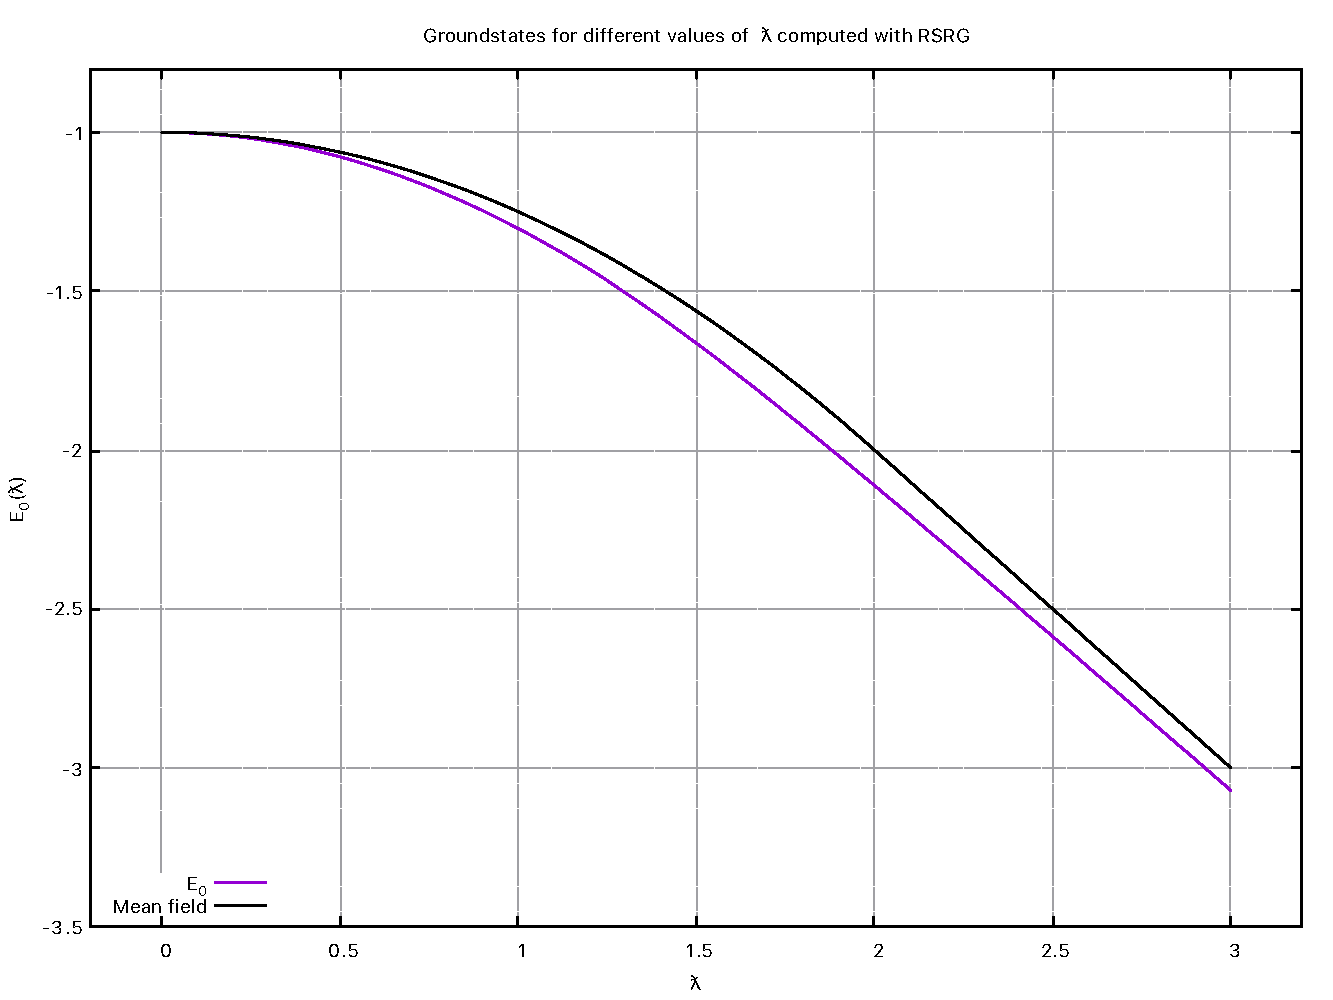
\includegraphics[width=.65\textwidth]{gr_st}\hfill
%%    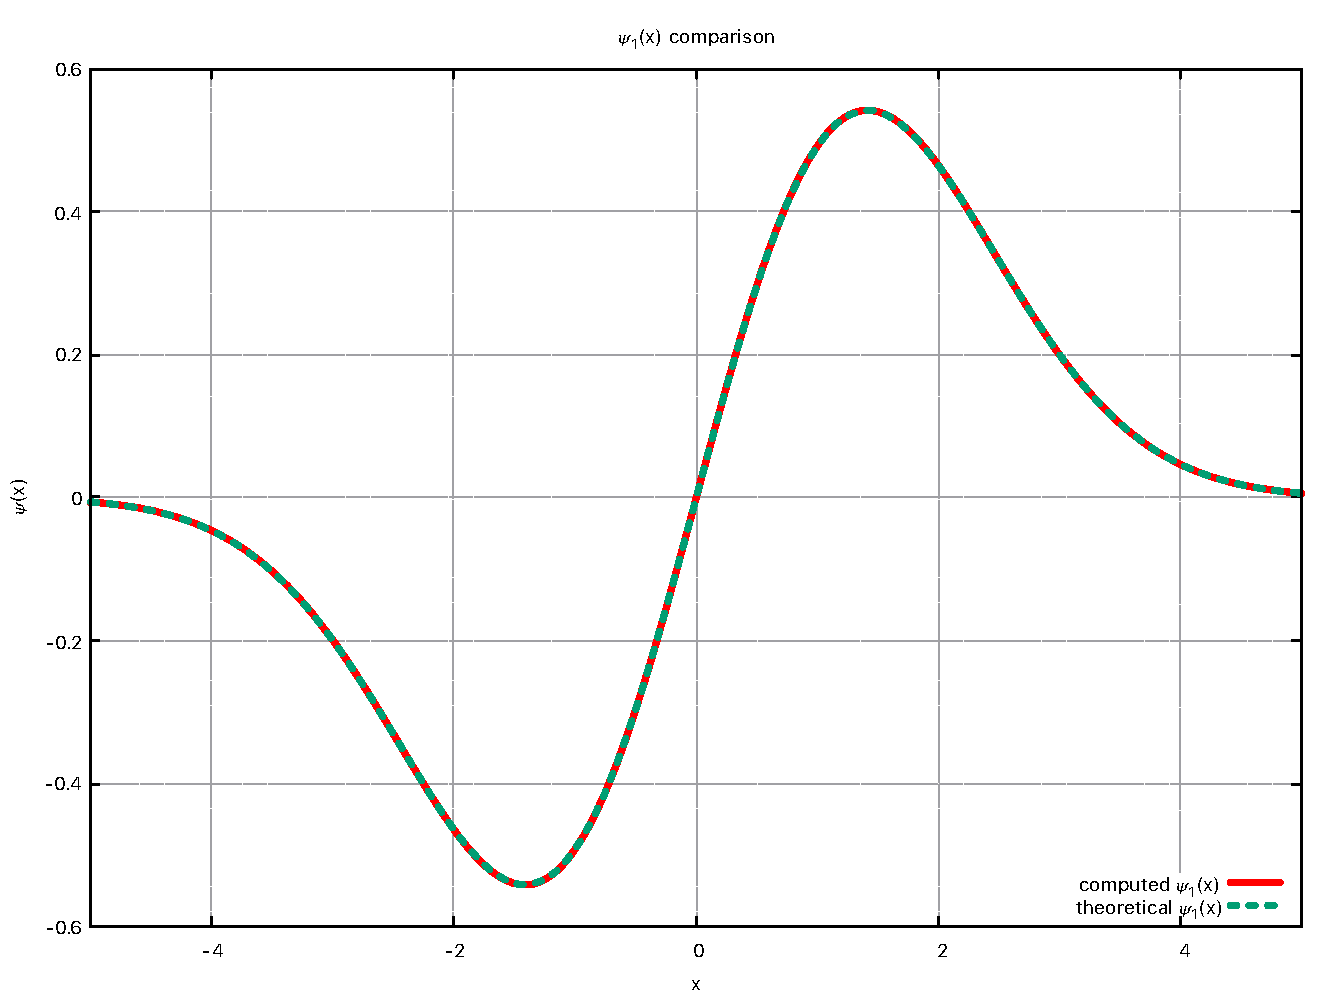
\includegraphics[width=.45\textwidth]{psi_1}\hfill
%%    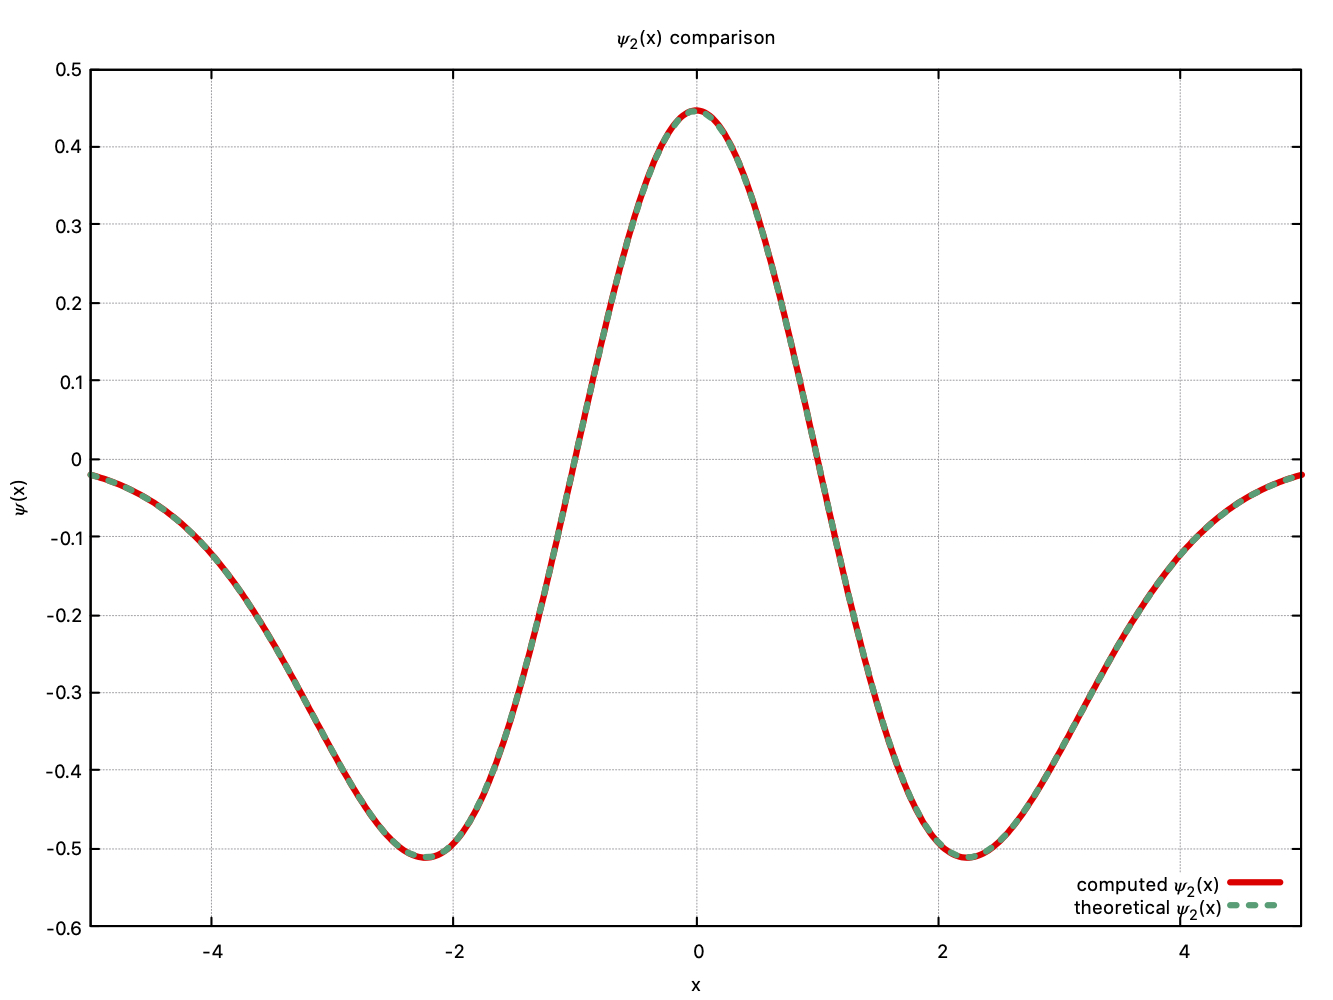
\includegraphics[width=.45\textwidth]{psi_2}
%%%    \\[\smallskipamount]
%%%    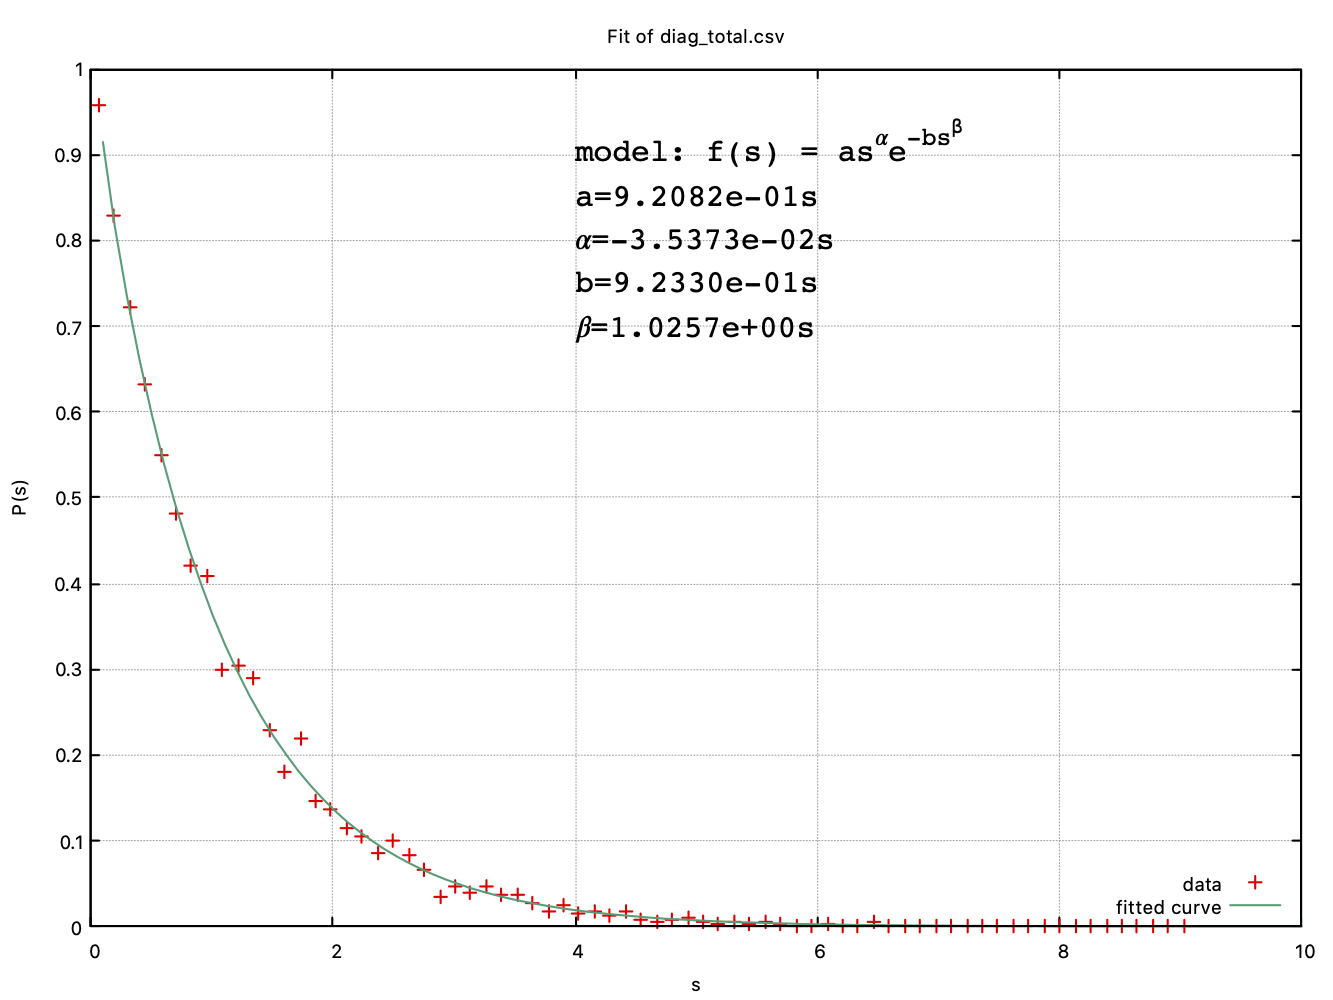
\includegraphics[width=.33\textwidth]{diag_total}\hfill
%%%    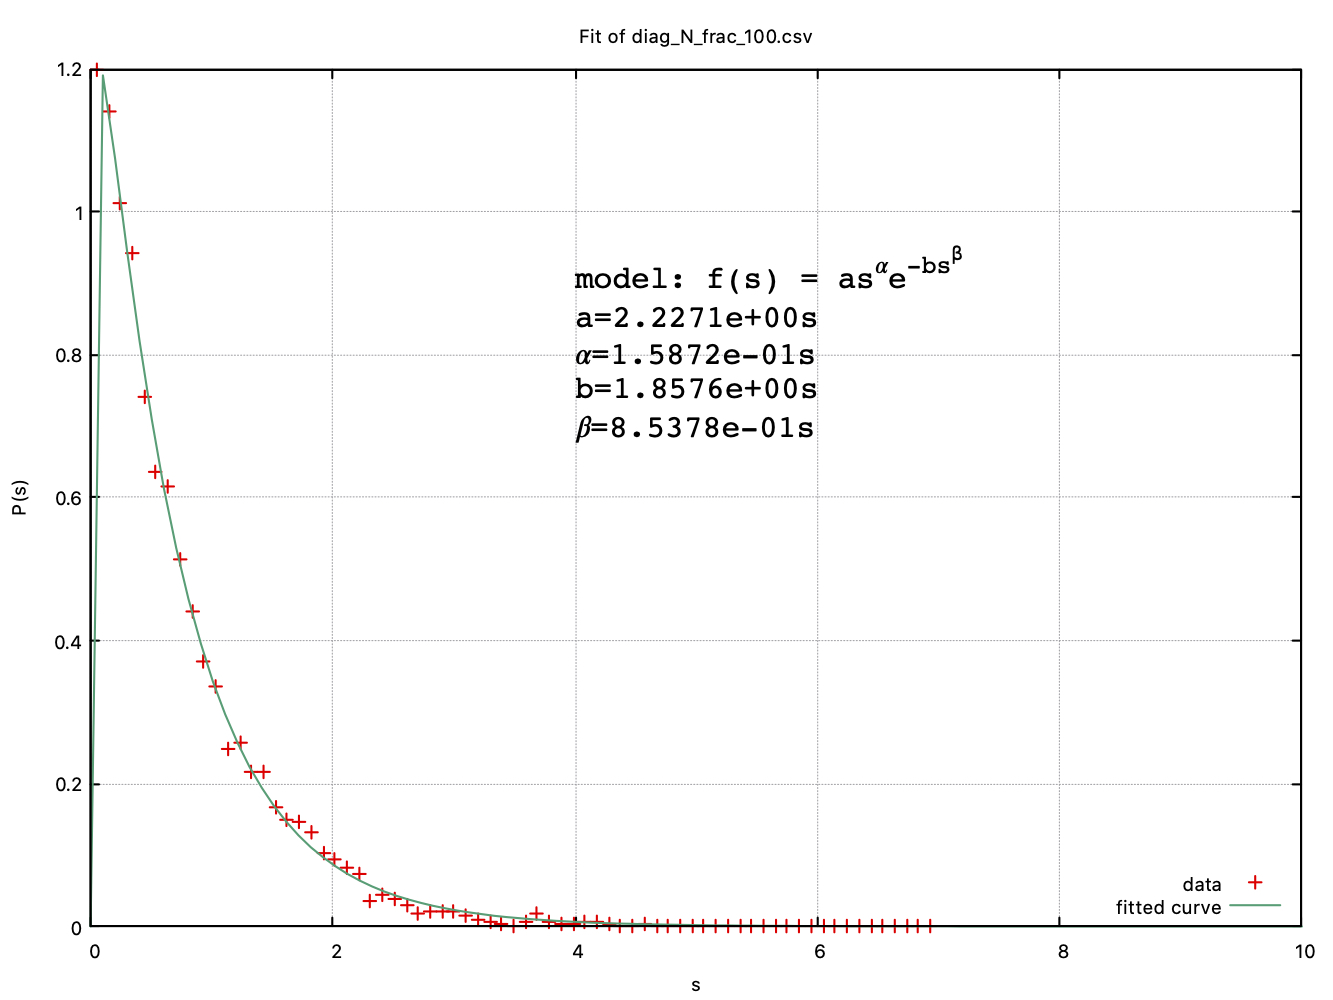
\includegraphics[width=.33\textwidth]{diag_N_frac_100}\hfill
%%%    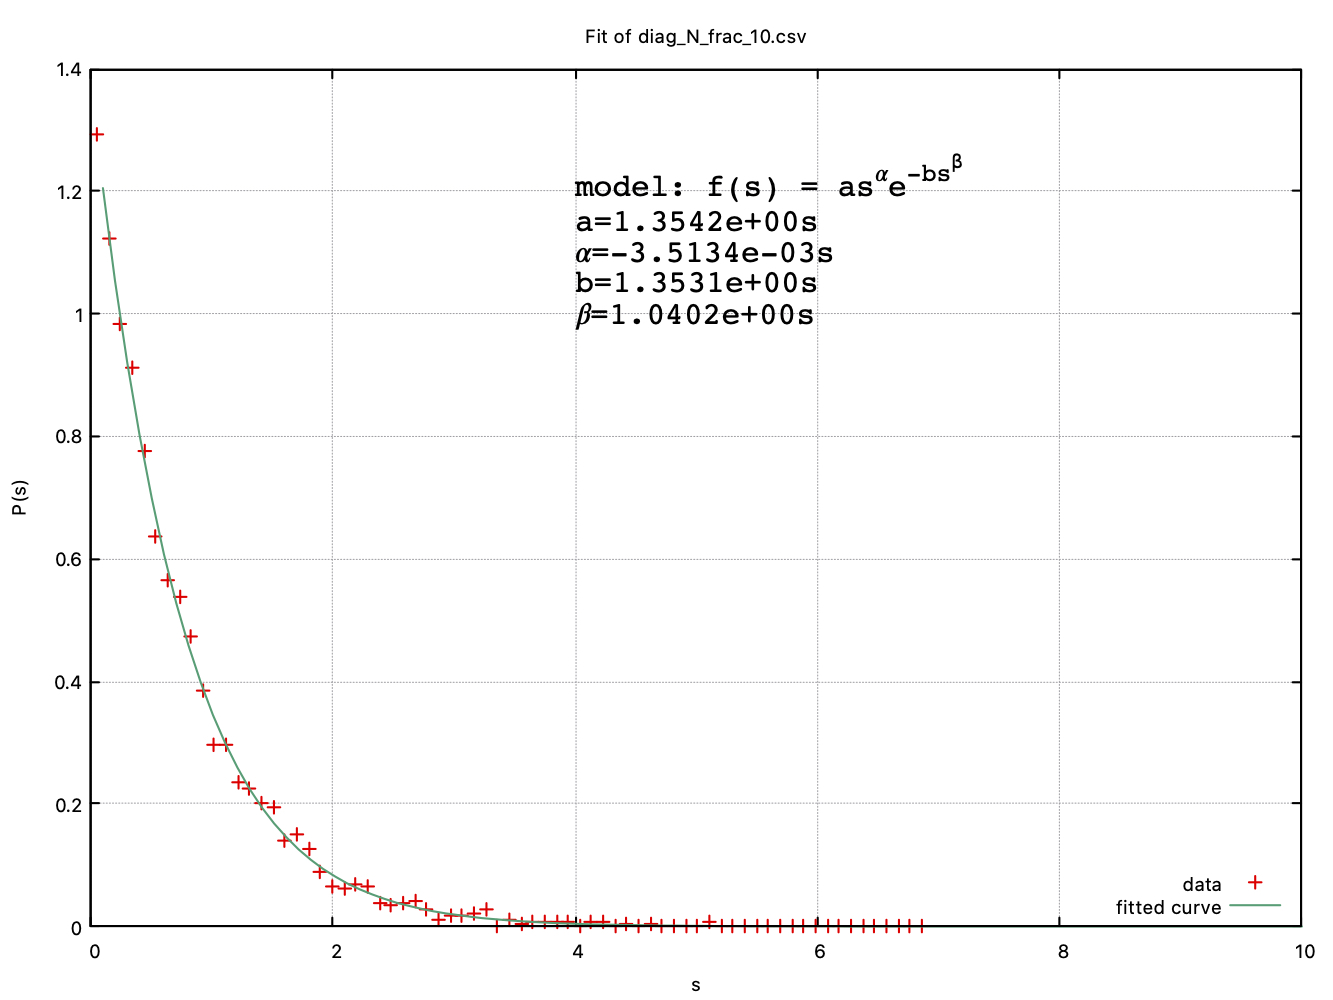
\includegraphics[width=.33\textwidth]{diag_N_frac_10}
    \caption{The ground states of a system of spins at thermodynamical equilibrium as a function of $\lambda$}\label{ground_states} computed by means of the RSRG algorithm
\end{figure}
%
%\begin{figure}[H]
%    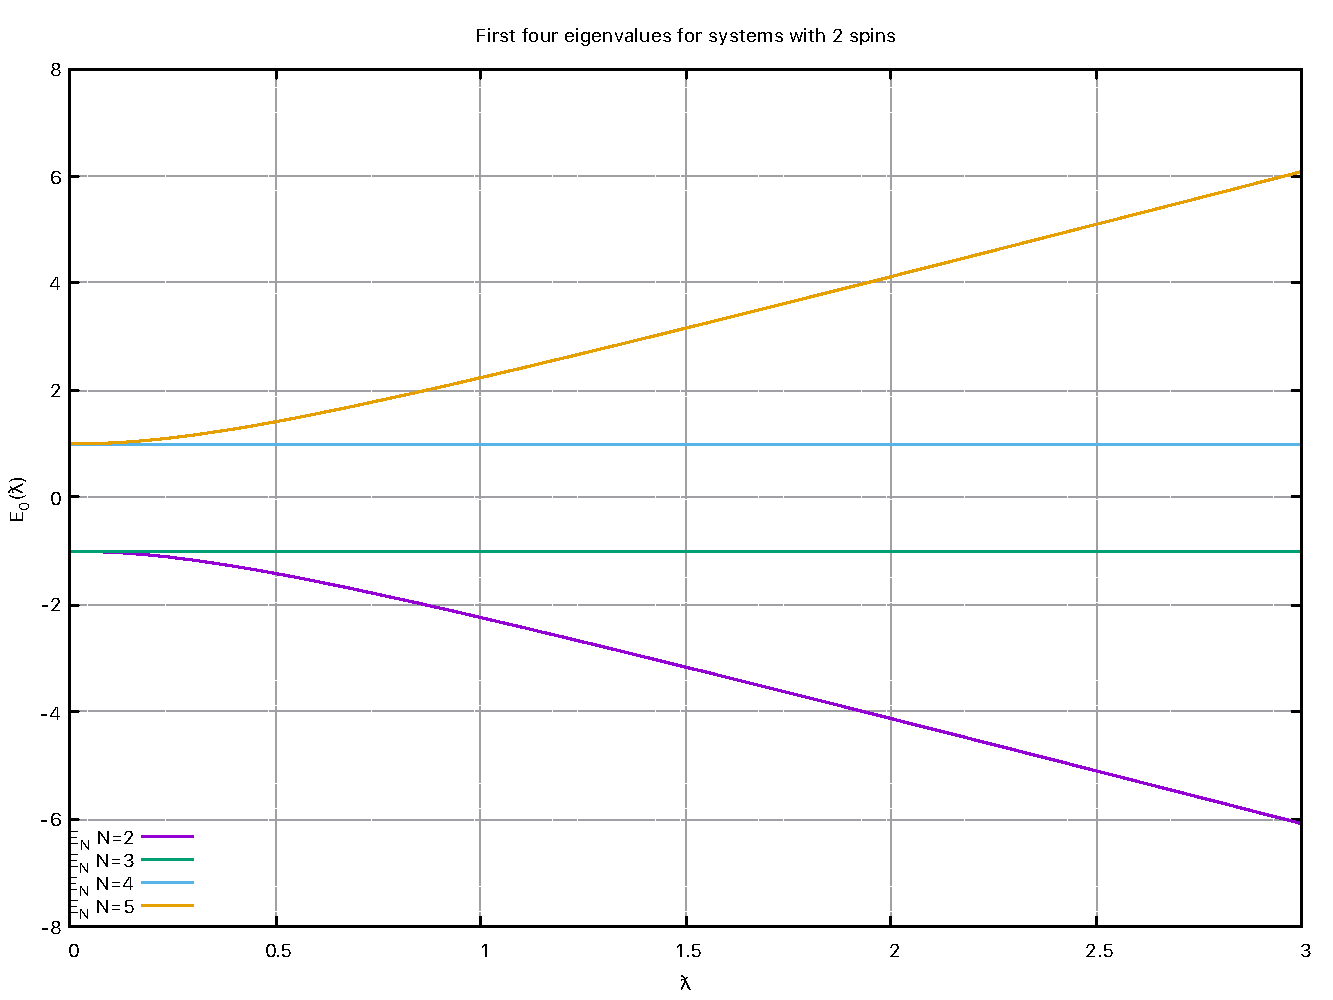
\includegraphics[width=.40\textwidth]{firstfour_2}\hfill
%    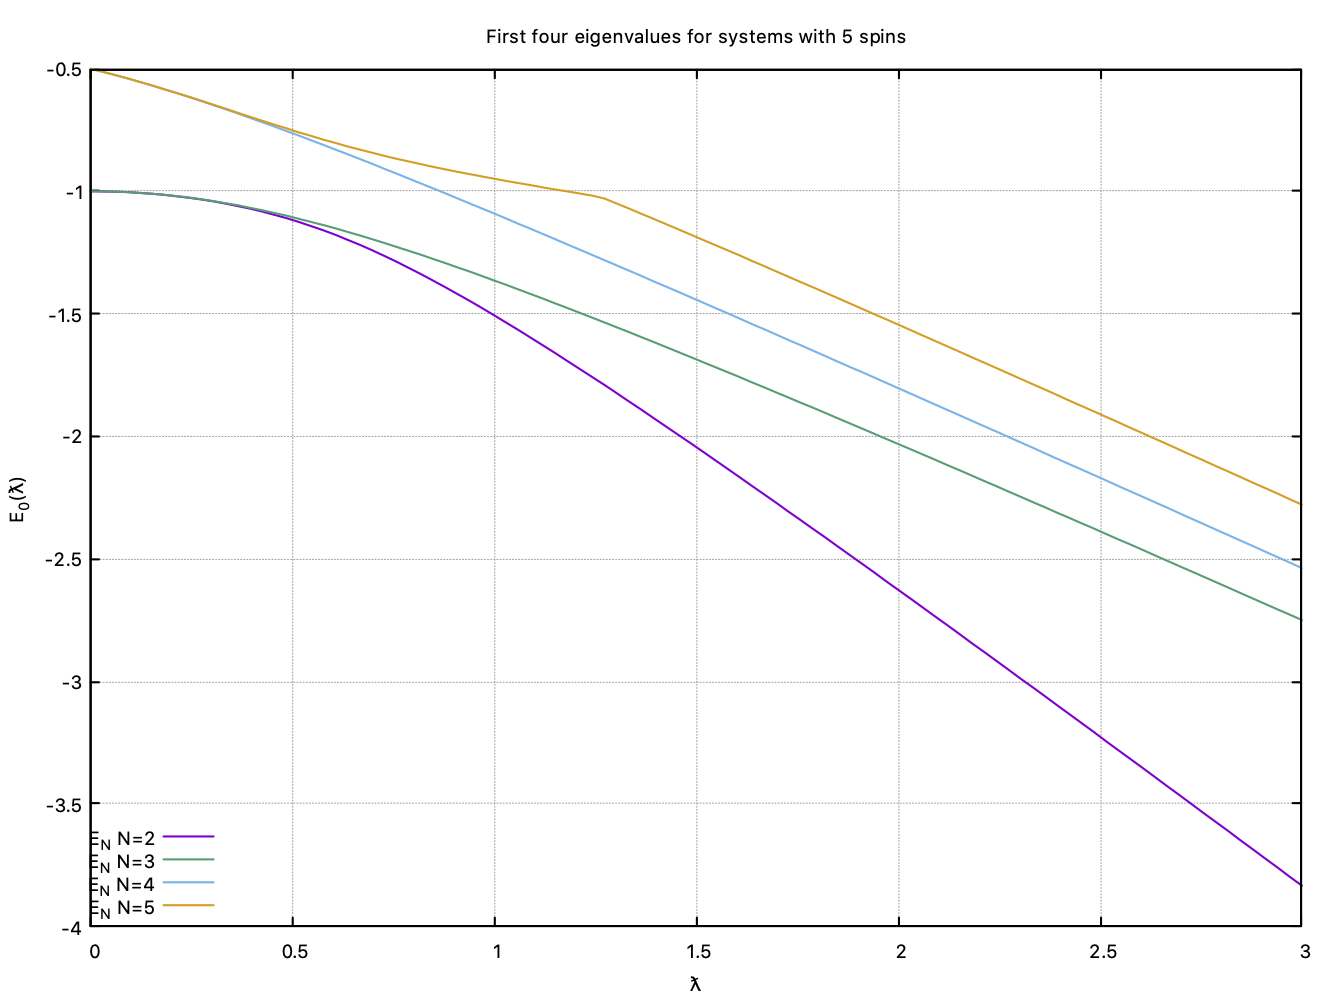
\includegraphics[width=.40\textwidth]{firstfour_5}\hfill
%%    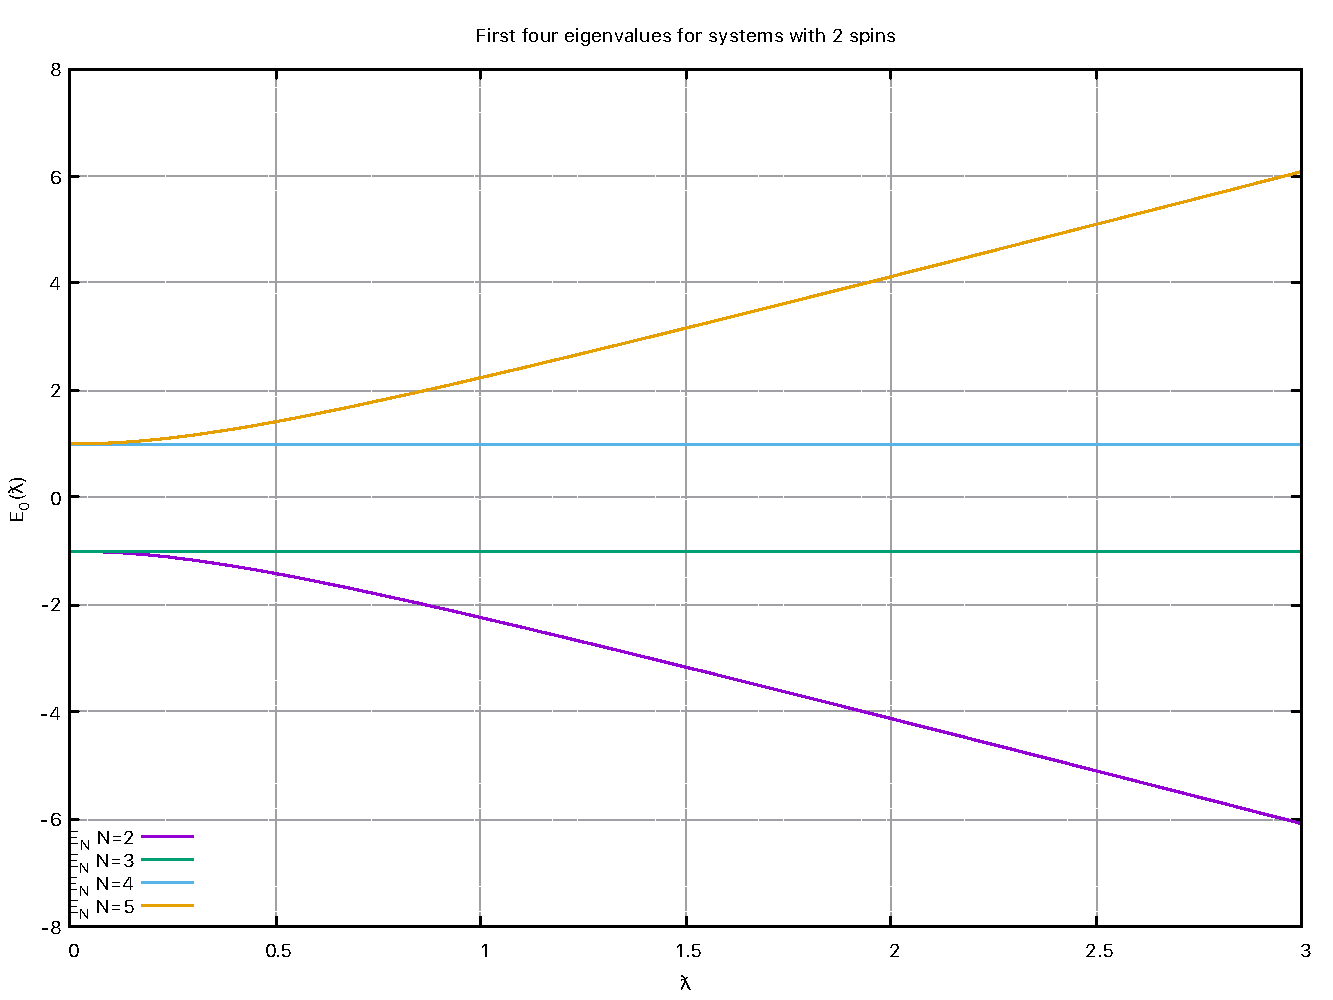
\includegraphics[width=.45\textwidth]{firstfour_2}
%    \\[\smallskipamount]
%    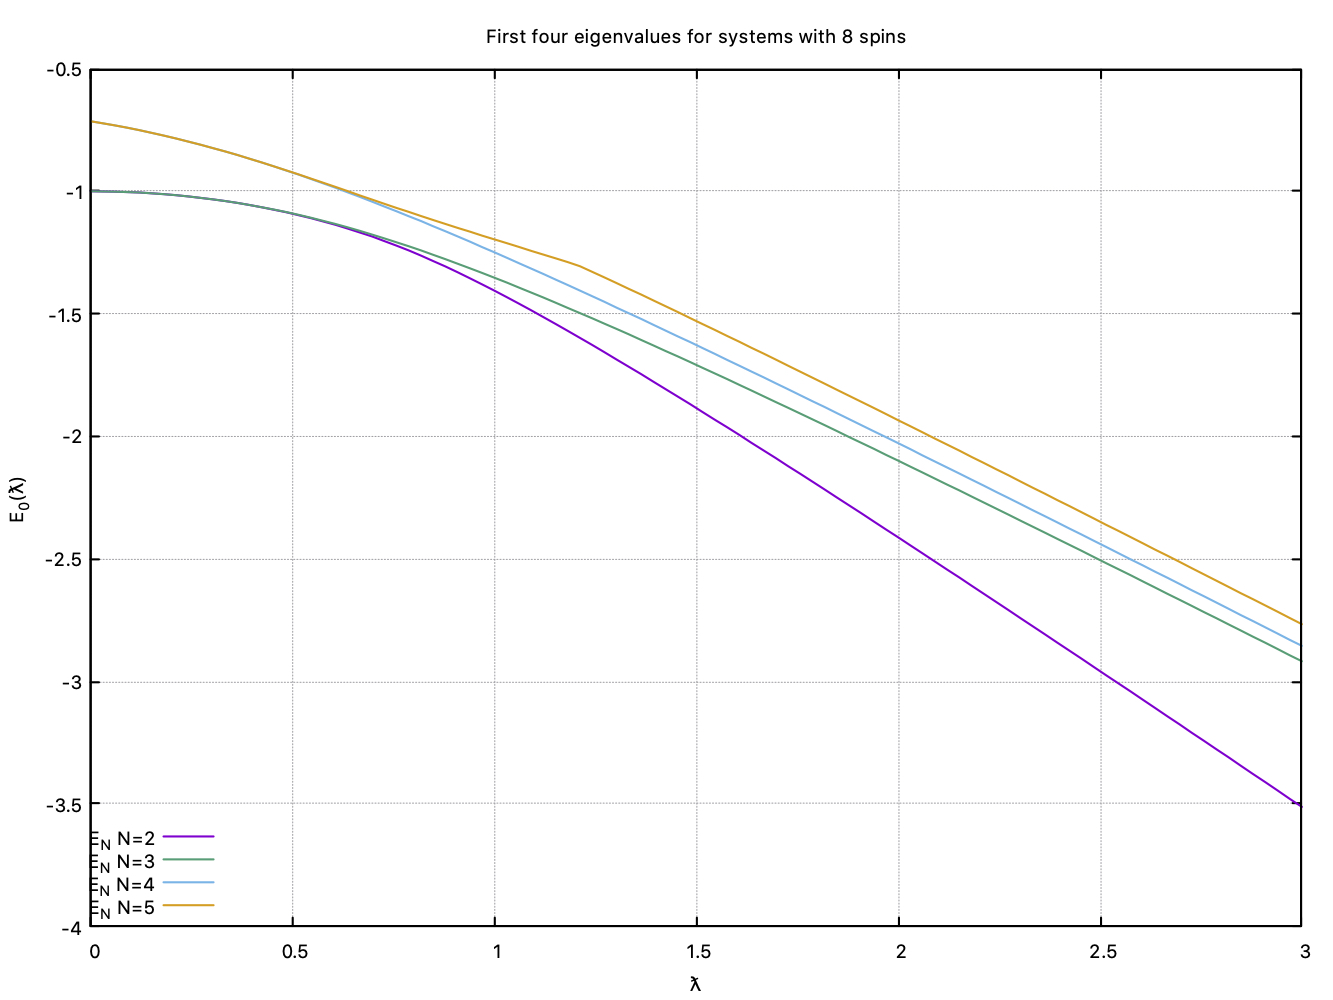
\includegraphics[width=.40\textwidth]{firstfour_8}\hfill
%    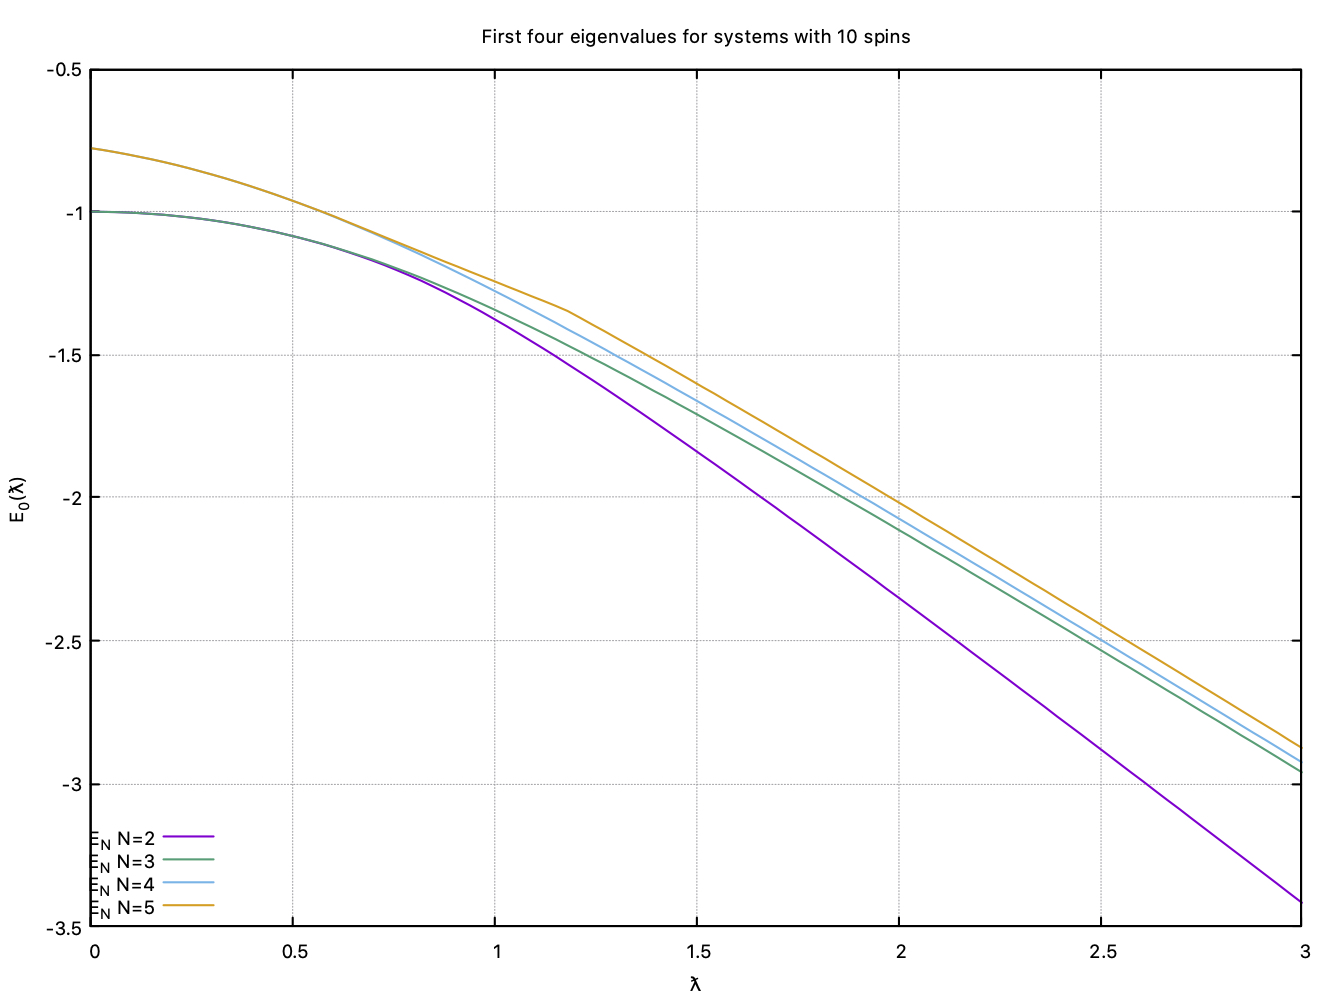
\includegraphics[width=.40\textwidth]{firstfour_10}\hfill
%%%    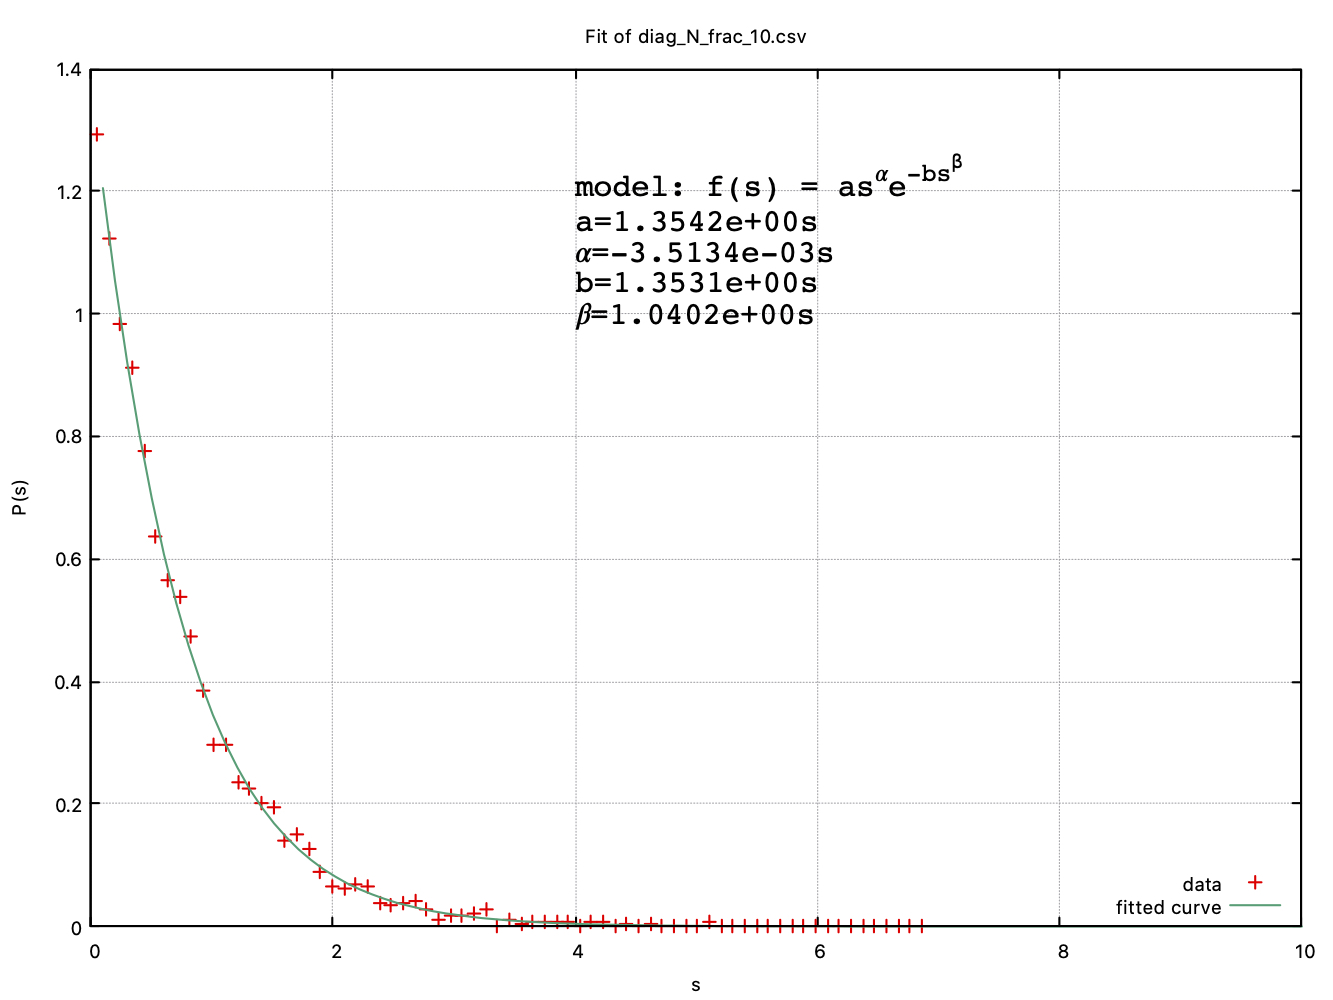
\includegraphics[width=.33\textwidth]{diag_N_frac_10}
%    \caption{the first 4 eigenvalues of the system for different values of $N$ as a function of $\lambda$}\label{fig:foobar}
%\end{figure}
%
\section{Self-evaluation}
I think the main objectives of the exercise are reached. I have learnt how to implement the RSRG algorithm to analyse the ground state of chains of spins with different number of particles.



\end{document}
